%%%%%%%%%%%%%%%%%%%%%%%%%%%%%%%%%%%%%%%%%%%%%%%%%%%%%%%%%%%%%%%%%%%%%%%%%%%%%%%%
%2345678901234567890123456789012345678901234567890123456789012345678901234567890
%        1         2         3         4         5         6         7         8

\documentclass[letterpaper, 10 pt, conference]{ieeeconf}  % Comment this line out
                                                          % if you need a4paper
%\documentclass[a4paper, 10pt, conference]{ieeeconf}      % Use this line for a4
                                                          % paper

\IEEEoverridecommandlockouts                              % This command is only
                                                          % needed if you want to
                                                          % use the \thanks command
\overrideIEEEmargins
% See the \addtolength command later in the file to balance the column lengths
% on the last page of the document
\usepackage[utf8]{inputenc}
\usepackage[english]{babel}
\usepackage{graphicx}
\usepackage{float}
\usepackage[center]{caption}
\usepackage{enumitem}
\usepackage[
backend=biber,
style=numeric,
sorting=ynt
]{biblatex}
 
\addbibresource{mybibliography.bib}
 




% The following packages can be found on http:\\www.ctan.org
%\usepackage{graphics} % for pdf, bitmapped graphics files
%\usepackage{epsfig} % for postscript graphics files
%\usepackage{mathptmx} % assumes new font selection scheme installed
%\usepackage{times} % assumes new font selection scheme installed
%\usepackage{amsmath} % assumes amsmath package installed
%\usepackage{amssymb}  % assumes amsmath package installed

\title{\huge \textbf{Cloud Service Benchmarking} 
\hfill \ \\
\LARGE{AWS DynamoDB vs. Google Spanner}
}
 
%\author{ \parbox{3 in}{\centering Huibert Kwakernaak*
%         \thanks{*Use the $\backslash$thanks command to put information here}\\
%         Faculty of Electrical Engineering, Mathematics and Computer Science\\
%         University of Twente\\
%         7500 AE Enschede, The Netherlands\\
%         {\tt\small h.kwakernaak@autsubmit.com}}
%         \hspace*{ 0.5 in}
%         \parbox{3 in}{ \centering Pradeep Misra**
%         \thanks{**The footnote marks may be inserted manually}\\
%        Department of Electrical Engineering \\
%         Wright State University\\
%         Dayton, OH 45435, USA\\
%         {\tt\small pmisra@cs.wright.edu}}
%}

\author{Denis Rangelov and Martin Dichev
\\
Group H}


\begin{document}


\maketitle
\thispagestyle{empty}
\pagestyle{empty}

%%%%%%%%%%%%%%%%%%%%%%%%%%%%%%%%%%%%%%%%%%%%%%%%%%%%%%%%%%%%%%%%%%%%%%%%%%%%%%%%
\section{INTRODUCTION}
The purpose of this report is to summarize and evaluate the measurements collected during the performance evaluation process of two Cloud-based services - DynamoDB \cite{DynamoWebPage} and Google Spanner \cite{SpannerWebPage}. It reveals the benchmarking setup used throughout the project as well as the reasoning behind the selected benchmarking approach. Apart from the current passage, the report comprises of 5 more sections. The first one is \textit{"Systems Under Test"} and illustrates the features that AWS DynamoDB and Google Spanner offer. In the \textit{"Benchmark Design"} section, the main focus is placed on the design objectives, the selected metrics, the workload and the benchmarking setup. The sections that follow present the results collected when measuring the performance of the benchamarking targets (i.e. AWS DynamoDB and Google Spanner) as well as our interpretation of these results. The report concludes with a brief overview of the encountered challenges during the project and also includes an assessment of the degree to which we managed to accomplish the envisioned project goals.





\section{SYSTEMS UNDER TEST}
\begin{center}
    \textit{"If you know the enemy and know yourself, you need not fear the result of a hundred battles" \\ 
    - Sun Tzu, The Art of War   }
\end{center}

Although the quote above is primarily intended as a playful and humorous way to open up the current section, there is a deeper meaning behind it. For the purposes of this writing, the idea of knowing your enemy can be translated as knowing well the systems one is trying to test. More specifically, when benchmarking a service is the main goal of a project, knowing the systems as close as possible is of crucial importance. Therefore, the current section is dedicated to summarizing some of the most well-known properties of DynamoDB and Google Spanner. Important to note here is that many of the properties of cloud services such as DynamoDB or Google Spanner remain "secret" for the general public. Therefore, despite our best efforts, it is possible that we might not be able to cover in much detail and with a complete accuracy how these systems operate behind the scenes. The information presented below was gathered by examining the reports from companies that actively use the services in question and also by reviewing the conference talks and papers the two service providers have published online.

\subsection{DynamoDB}
DynamoDB is a scalable, fully managed NoSQL cloud database service. It supports key-value and document data structures. Although it is known that Amazon built DynamoDB on top of principles used in their previous Dynamo \cite{DeCandia:2007:DAH:1323293.1294281} and SimpleDB projects, DynamoDB's architecture still remains a black box for its users \cite{Allthings}. However, according to the information provided by Werner Vogels \cite{Allthings} - CTO and vice president of Amazon - Amazon DynamoDB stores data on Solid State Drives (SSDs) and by default works within one AWS region and replicates data to 3 separate availability zones. Cross-Region Replication is also possible by using the Global Tables feature which links identical tables in different regions through an automated asynchronous replication mechanism. In terms of the CAP theorem, DynamoDB is an AP (Available and Partition-tolerant) database. It supports only eventual write consistency, but for reads the user can choose between eventual and strong consistency (trading off availability). 

\subsection{Google Spanner}
Cloud Spanner is a strongly consistent, highly available, globally distributed, synchronously-replicated database \cite{SpannerWebPage}. Its main focus is managing cross-datacenter replicated data while still trying to maintain the more traditional SQL database properties. To clarify, Google Spanner aims at providing both system availability and data consistency, by combining SQL and NoSQL traits and can therefore be classified as a NewSQL database. "NewSQL" is a term first coined by Michael Stonebraker in an article from 2011 \cite{newsql}. In one of the more recent papers on NewSQL (2016), the term is described as:
\textit{"Our definition of NewSQL is that they are a class of modern relational DBMSs that seek to provide the same scalable performance of NoSQL for OLTP read-write workloads while still maintaining ACID guarantees for transaction"} \cite{Pavlo:2016:WRN:3003665.3003674}. \par
Going back to Spanner, the data inside is stored in tables with a well defined schema and a SQL-based query language is provided. Spanner's stance regarding The CAP Theorem is intriguing, because of its claim to be both consistent and highly available, but technically unlike the AP DynamoDB, Spanner is a CP(Consistent and Partition-tolerant) system \cite{SpannerWebPage}. While the DynamoDB internals remain hidden from us, Google provides some information about how Spanner operates behind the scenes: \par
Spanner partitions database tables into contiguous key ranges called splits. In their official documentation, Google describes the management of these splits as follows:
\textit{"A single machine can serve multiple splits, and there is a fast lookup service for determining the machine(s) that serve a given key range. Each split is replicated to multiple machines in distinct domains. The consensus problem solving Paxos algorithm manages consistent replication to the different copies of the split. In Paxos, as long as a majority of the voting replicas for the split are up, one of those replicas can be elected leader to process writes and allow other replicas to serve reads."} \cite{SpannerWebPage}.
Like most databases supporting ACID properties, Spanner uses 2PC and 2PL to ensure isolation and strong consistency. Furthermore Spanner offers two difficult to implement in a distributed database features: it provides externally consistent reads and writes, and globally-consistent reads across the database. External consistency is an even more strict property than strong consistency and Google describes it as follows:
\textit{"Cloud Spanner provides clients with the strictest concurrency-control guarantees for transactions, which is called external consistency. Under external consistency, the system behaves as if all transactions were executed sequentially, even though Cloud Spanner actually runs them across multiple servers (and possibly in multiple datacenters) for higher performance and availability. In addition if one transaction completes before another transaction starts to commit, the system guarantees that clients can never see a state that includes the effect of the second transaction but not the first. Intuitively, Cloud Spanner is semantically indistinguishable from a single-machine database."} \cite{SpannerWebPage}.
These features are possible, because Spanner assigns globally-meaningful commit timestamps to its transactions thanks to its novel TrueTime technology - Google's synchronized clock. For any two transactions T1 and T2 (even if on opposite sides of the globe) holds Spanner's external consistency invariant: if T2 starts to commit after T1 finishes committing, then the timestamp for T2 is greater than the timestamp for T1. TrueTime's references are GPS and atomic clocks. It uses the two forms of time keeping, because of their uncorrelated ways of failure. Thanks to the timestamps clients can do globally consistent reads across the entire database without locking (reads do not acquire locks in read-only transactions), while typically when an application wants to read the most current data from a traditional database that uses strict 2PL, the database will acquire a read lock on the data. To conclude Spanner uses two-phase commit to achieve serializability, but it uses TrueTime for external consistency and consistent reads without locking. \par
With all that being said, we cannot be completely sure that the details that Google exposes are the precise way in which Spanner is working internally. The configuration options are another aspect of spanner that does not offer a lot of freedom. Therefore, this store still remains somewhat close to "black-box" model that DynamoDB follows.

\section{BENCHMARK GOALS AND DESIGN}
The main objective of this section is to briefly describe how we address the general benchmark design objectives, what performance metrics we decided to focus on and also what type of workloads we choose to utilize. That being said, the first important discussion to kickoff the current section is the benchmarking goal that we worked on throughout the project.  

\subsection{Benchmarking Goal}
In terms of the benchmarking goal, we decided to aim our attention at the following research question(s): 
\begin{itemize}
    \item What is AWS DynamoDB and Google Spanner’s write performance in terms of latency when both stores are introduced with update heavy workloads? 
    \item How does the database record size affect the write latency of the two stores?  
\end{itemize}
The decision to examine these benchmarking scenarios is based on the tendency that many of the modern web applications are handling a huge amount of OLTP workloads (i.e. insert/update/delete requests). Therefore, we decided to apply update heavy stress on the two benchmarking targets which - at least in our experience - is a workload that occurs often times in practice and in real-life use cases (e.g. updating the items in your shopping cart, changing the status in your social media profile, etc.). To be completely honest, the workloads used throughout the project are synthetic (more on that in later sections) which means that it is really impractical to associate the applied workloads with a specific application scenario. Rather, we will use the update heavy workload to test \textit {"small isolated features"} \cite{StefanTaiBook} such as the write performance (especially for different record sizes) of the two data stores.


\subsection{Benchmarking Tool}
To help us answer the research questions mentioned above, we choose a benchmarking tool called \textit{Yahoo! Cloud Serving Benchmark (YCSB)} \cite{Cooper:2010:BCS:1807128.1807152}. Among the reasons that we decided to work with YCSB are:
\begin{itemize}
    \item It has out-of-the box drivers for both DynamoDB and Google Spanner  
    \item It offers a large number of predefined workloads to choose from
    \item It has a multitude of "switches and knobs" that we can turn on and off based on the needs of the project
    \item It allows us to scale the workloads effortlessly
    \item It has an awesome documentation 
\end{itemize}
With this in mind, throughout the project we did some additional testing with workloads that are indirectly related to the research goals presented in the beginning of the section. The collected measurements allowed us to acquire a broader perspective of what are the strengths and weaknesses of the systems under test and for this reason we will briefly discuss them in the later sections of this report.

\subsection{Benchmarking Metrics}
As mentioned in the "Benchmarking Goals and Design" section, the goal of the experiments conducted in the scope of this project is to collect measurements of the write performance of DynamoDB \cite{DynamoWebPage} and Google Spanner \cite{SpannerWebPage}. To achieve that goal, as a performance metric we examined the write/update \textit{latency} measured in milliseconds. It is important to mention here that we assumed a client's perspective throughout the benchmarking sessions. The reasoning behind this decision is not only based on the task description (it was suggested to do so in the assignment sheet) but also on the fact that this perspective includes the roundtrip time to the collected measurements. As mentioned in the "Cloud Service Benchmarking" book by Prof. Tai \cite{StefanTaiBook}, the round trip time has an important impact on the overall latency (network delays are not to be underestimated) and therefore it was a logical choice to adopt the client's perspective in our benchmarking setup.

\subsection{Benchmarking Setup}
Our experience while working on this project, led us to the conclusion that when it comes to benchmarking cloud services, choosing the correct setup is one of the most challenging aspects of the task at hand. To be precise, there is a large variety of parameters that were relevant for the benchmarking experiments and could not be neglected. Among the most prominent ones (especially for DynamoDB and Spanner) are the geolocation of both - the benchmarking client and the SUTs, the provisioned resources and the data distribution. We will break down the each of these individually below:
\\
\\
\underline{Geolocation of the Benchmarking Client:}
\\
In the \textbf{ideal case}, the client should be geo-distributed so that the benchmark setup can look as close as possible to a real application scenario (e.g. multiple users in different parts of the world trying to access a web service). Unfortunately, the benchmarking client used throughout the project does not support geo-distribution, but instead it was deployed only in one region. The main reason for the usage of a non-distributed client setup is that we don't have the necessary coordination mechanisms among the YCSB clients, that can ensure that the distributed load will "hit" the SUT's in the intended way. One example that simultaneously supports and illustrates this claim is presented in the Cloud Service Benchmarking book \cite{StefanTaiBook}, where the authors point out that for loads that try to target a specific range of keys (e.g. triggering a hot-key problem), using YCSB in a distributed manner might not actually produce the desired stress on the system because of the probability distributions YCSB uses when generating the workloads. \par
That being said, even with a non-optimal single client deployment, there is still one important point to be considered - which region to deploy the benchmarking client to? The short answer is that we deployed the benchmarking client on one of our local machines here in Berlin. The long answer, on the other hand, is that when we deployed the benchmarking client on a EC2 instance in another region, we observed a very strange behavior. In particular, the EC2 was giving an unfair advantage to DynamoDB (higher throughput) compared to Spanner. It is really difficult to make a conclusive statement, if this behavior is the norm, but it is very likely that services in the AWS ecosystem communicate with each other in a more efficient manner because of either software or hardware optimizations. For instance, one possible (although speculative) explanation for these results could be that AWS uses high speed interconnects between their data centers. \par
With this context in mind, we decided to use a more neutral environment for the benchmarking client and that is why we ran the client from our local machine.
\\
\\
\underline{Geolocation of the Benchmarking Targets:}
\\
Similar to the geolocation of the benchmarking client, in the \textbf{ideal case}, both SUTs should be deployed in a distributed fashion so that the benchmarking use case looks very close to a real life scenario. However, to deploy a fully geo-distributed Spanner instance (i.e. with replicas in Europe, Asia and USA), the cost is 9\$/hour. Even with the free credits, since we ran the experiments for a relatively long time to ensure reproducibility, it was impossible for us to keep up with the enormous costs (we even used a full-fledged account with 300\$ free credits but it was still too expensive to keep the Spanner instance running). \par
On the DynamoDB side, things did not go so well either. According to our research, the geo-distributed deployment of DynamoDB is called "Amazon DynamoDB global table". After trying to initialize one such instance, we got an Email by Amazon saying that there is \textit{"insufficient replicated write capacity units"} for the free-tier and the student accounts. \par 
Finally, since the geo-distributed deployment did not work as expected, we deployed both data stores in only one -  the eu-west-2 (London) - region so that each one of them is equally far from the benchrmaking client's location.
\\
\\
\underline{Provisioning resources:}
\\
In terms of resources, the two stores do not offer that many configuration options. In fact, both DynamoDB and Spanner are mostly black-box systems that leave almost no decisions for the customer to make. Outside of the geo-distribution mentioned above, there is only one more option left to configure for both systems. With Spanner this option is the number of nodes which is not to be confused with the number of replicas. In the Spanner documentation this detail is explained as follows : \textit{"If you need to scale up the serving and storage resources in your instance, add more nodes to that instance. Note that adding a node does not increase the number of replicas (which are fixed for a given configuration)"} \cite{SpannerInstances}. Instead of speculating what "scale up the serving and storage resources" precisely means, we just left the default settings which spawns only one Spanner node. \par 
With DynamoDB the only option that we could set is the minimum/maximum provisioned read/write capacity units. Since we did not change the default instance settings for Spanner, we decided to do the same with DynamoDB. In the \textbf{ideal case} we would have definitely provisioned both stores in the closest possible manner in terms of resources. Unfortunately, by operating as black-box, these systems leave almost no space for customer configuration and that's why we decided to leave the data stores provisioned with the default provider's settings.
\\
\\
\underline{Data distribution}
\\
Since the benchmarking targes are distributed data stores, they allow the customer/developer to decide how the data will be distributed across the network. For DynamoDB the data partitioning is determined by the partition key chosen by the customer at the table initialization. With Spanner it is determined by the primary key also chosen by the customer when defining the database schema. To make the two deployments as similar as possible, we chose the same partition key for both stores.

\subsection{Assesment of the Benchmark Design Objectives}
According to S. Tai, D. Bermach and E. Wittern, there are five general benchmark design objectives - relevance, reproducibility, fairness, portability and understandability \cite{StefanTaiBook}. In this subsection, we will briefly assess how our benchmark performs based on these objectives.
\\
\\
\underline{Relevance:}
\\
The envisioned benchmark targets the write performance of DynamoDB and Google Spanner in terms of latency. Since OLTP (i.e. insert/update/delete) workloads are common in today's web applications \cite{OLTp} (e.g. e-commerce stores) , we can safely say that using a update heavy workload addresses a realistic enough scenario. Additionally, it is reasonable to assume that real-life use cases that include a huge amount of write operations are here to stay in the future. Taking this information into account, we can conclude that the envisioned benchmark is relevant.
\\
\\
\underline{Reproducibility:}
\\
To ensure reproducibility, we ran the prepared experiments multiple times at different times of the day. Figures \ref{fig:workloadA_morning} and \ref{fig:workloadA_night} illustrate the the results collected from doing so. Based on our observations, both stores perform very similarly and they always produce \textbf{approximately} the same results. Therefore, we will not do a more in-depth comparison between the performance based on the time of the day. That being said, although in the Cloud there is always the possibility for unstable behaviour, we can safely say that at least at the time of this writing the benchmark satisfied the reproducibility as a design objective.
\\
\\
\underline{Repeatability:}
\\
Since YCSB as a benchmarking tool operates with synthetic workloads, the benchmark we developed for the project does not fulfill the repeatability design objective. The reason is that with synthetic workloads, there is always a random element attached to each individual benchmark run which hinders us from repeating the \textit{exact} same experiment multiple times.
\\
\\
\underline{Fairness:}
\\
In general, the benchmark is not completely fair. The reason for that is that most modern NoSQL and NewSQL stores are optimized for write heavy workloads. This means that if the benchmark experiment is executed on a traditional SQL store (e.g. Postgres, MySQL, DB2, etc.), this might put the NoSQL stores in a advantageous position. However, if we take a step back and focus only on DynamoDB and Spanner, the benchmark in its current form does not give any advantage to either of the stores. Therefore, we can conclude that in the more general cases the benchmark is not treating all data stores in a fair manner, but in the scope of the project, the benchmark treats DynamoDB and Google Spanner fairly.
\\
\\
\underline{Portability:}
\\
With the help of the YCSB tool, it was not difficult to ensure portability for the benchmark. YCSB offers an enormous number of adapters for almost all popular cloud-based (and not only) data stores. This means that the benchmark can be executed against a large number of systems (which is also the definition of "portability" presented in "Cloud Service Benchmarking" \cite{StefanTaiBook}) and DynamoDB and Google Spanner are no exception.

\subsection{Workload Types}
The type of the workloads used throughout the project can be examined from multiple perspectives. Firstly, the workloads that YCSB offers are \textbf{synthetic} by nature - which explains why the workloads we applied are also synthetic. As for the granularity level of the benchmark is concerned, we are using \textbf{micro-benchmarks}. The explanation is that as we already mentioned in the "Benchmarking Goals" subsection, we are testing a relatively small, highly specific feature of both data stores. Lastly, in terms of the workload generation model, based on our understanding, YCSB uses the "closed" model, although in practice it is not the most \textit{"realistic"} approach \cite{StefanTaiBook}.

\section{Benchmark Execution}
The purpose of this section is to describe the process of conducting the experiments planed in the scope of the project. Some of the aspects that are relevant for this section, were already discussed in section "Benchmark Goals and Design" (e.g. \textbf{provisioning of resources}, \textbf{geolocation} of the benchmarking clients and SUT's). Therefore they will not be explicitly repeated unless necessary.

\subsection{Experiment Phases}
The experiments we conducted as part of the assignment consist of multiple phases - pre-loading, warmup, actual experiment phase, data collection and cleanup. Each one of these is described below:
\\
\\
\underline{Pre-loading Phase:}
\\
Since we are benchmarking two data stores, the pre-loading phase is of crucial importance. Therefore, during this phase we loaded the records used during the actual experiments. The duration of the pre-loading phase varied drastically based on the workload settings. For instance, with our initial setup, we tried to insert 10 000 000 records which resulted in an estimated loading time of 3 days for DynamoDB. Therefore we reduced the number of records to reach a more reasonable loading time of around 45 minutes up to 1 hour - i.e. we conducted the experiments with 30 000 records. Also, during this phase we discovered a feature of Google Spanner which really made it stand out from DynamoDB and namely - Spanner offers batch inserts. Putting this feature into use, made Spanner's pre-loading phase from hundred to a thousand times shorter than the pre-loading phase of DynamoDB. 
\\
\\
\underline{Warmup Phase:}
\\
The warmup phase we used was rather simplistic. Instead of running the experiment with 50000 operations as for the full-fledged experiment, we scaled the request count down to 1000 operations. As suggested by the authors of the "Cloud Service Benchmarking" book in chapter 9 \cite{StefanTaiBook}, we executed the actual experiment immediately after the warmup was over, so that we can avoid periods of idleness in-between the two phases.
\\
\\
\underline{Experiment Phase:}
\\
The only noteworthy detail for the experiment phase were the settings used with each individual run. For the purposes of answering the research questions introduced in section "Benchmark Goals and Design", we used the following configuration:
\begin{itemize}
    \item Every experiment included 30 000 operations
    \item Update heavy workload with 80/20 write-to-read ratio
    \item Duration of each individual experiment - 25 minutes
    \item The size of the database record fields varied from experiment to experiment (from 100 bytes up to 1000 bytes)
    \item Each database record consists of 10 fields. Therefore the approximate size of a record is equal to:
    $$
    (field size) * 10
    $$
\end{itemize}
Also, to ensure that DynamoDB and Google Spanner behave similarly during different times of the day we ran the experiments in the morning, in the afternoon and late at night. The results of these experiments as well as the behavior of the two stores are included in the "Results" section. \par
Lastly, outside of the experiments directly related to the research questions, we collected additional measurements that reveal an interesting behavior from the two stores. Although these results are indirectly related to the benchmarking goals for the project, we decided to include some of the more interesting observations at the end of the "Results" section.
\\
\\
\underline{Data Collection Phase:}
\\
Since we ran the benchmarking client on a local machine, this phase was relatively effortless. We used the most simplistic data collection strategy and stored the collected measurements in a local file. After the experiment was over, we manually filtered the relevant data and organized it in a Excel spreadsheets for further processing.
\\
\\
\underline{Cleanup Phase:}
\\
To return both data stores to their original state (i.e. the state before running an experiment) we took the most unsophisticated, brutal, cruel, crude and uncivilized approach. Jokes aside, instead of overthinking it, we decided to just delete all tables, records and traces of the experiment altogether after each experiment is over. This way we go through all the phases described here (from pre-loading to cleanup) for each individual run and we end up with a "clean slate". Although this might not be the most elegant way to clean the benchmarking setup, it saved us a lot of time in dealing with automation tools and alternative fine-grained cleanup scenarios. 

\section{Results}
After describing our setup, the applied workloads, the executed benchmarking phases, the specific configuration for the "Experiment Phase", here, we will finally summarize the results acquired during the benchmarking experiments. The section opens up with the write performance measurements and our interpretation of them. All in all, we executed 4 benchmarks - with field size of 100, 300, 500 and 1000 bytes. However, these 4 benchmarks do not include the ones executed at different times of the day (to establish if the SUTs show stable results throughout the day) and the ones that are only indirectly affecting the write performance. \par
That being said, at the end of the section, we will include a brief summary of some additional experiments that we found interesting during the project.

\subsection{Update Heavy Workload (field size 100 bytes):}
Figures \ref{fig:workloadA_size100} and \ref{fig:boxplot_size100} present the results of executing our benchmark with the default record size of 1kB (i.e. field size 100 bytes).
\begin{figure}[h]
\centering
\fbox{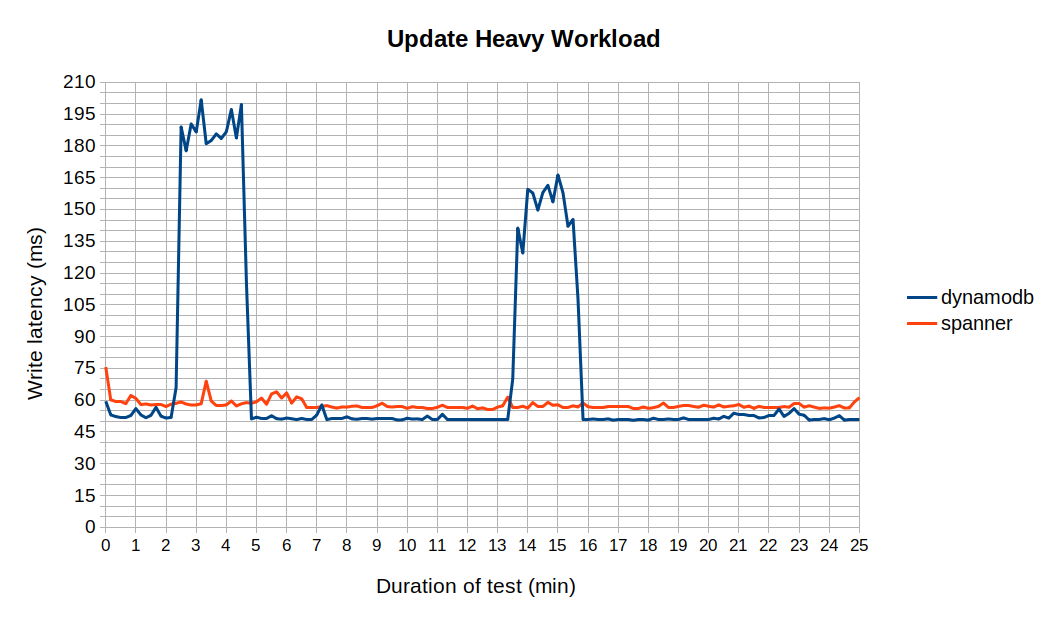
\includegraphics[width=0.47\textwidth]{workloadA.png}}
\caption{Line Chart for Executing Update Heavy Workload (field size 100 bytes)}
\label{fig:workloadA_size100}
\end{figure}  
 
\begin{figure}[h]
\centering
\fbox{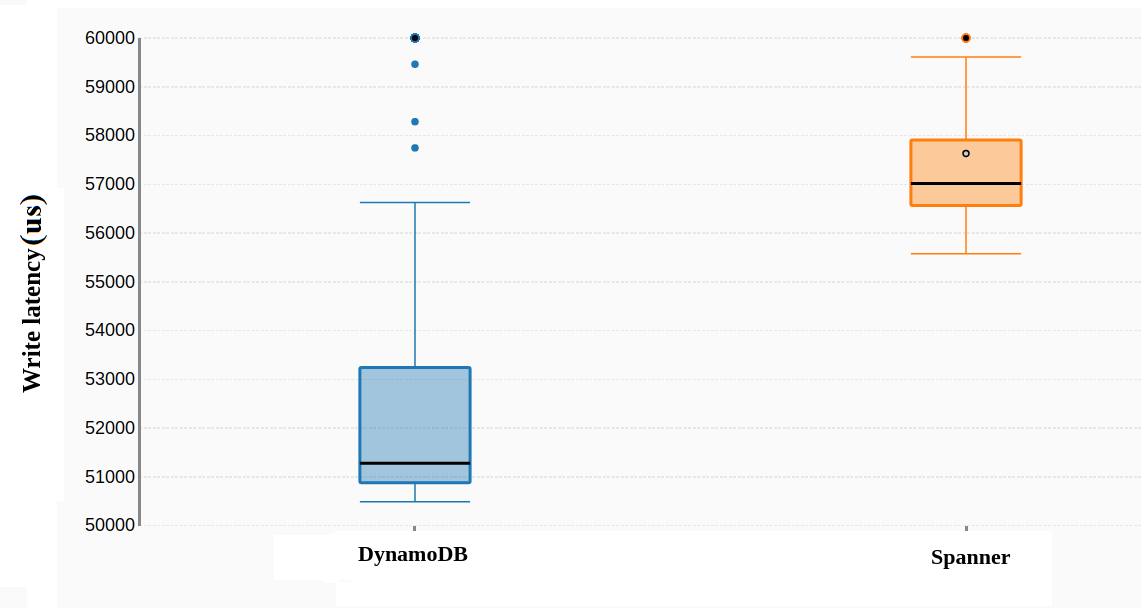
\includegraphics[width=0.47\textwidth]{boxPlotA.png}}
\caption{Box Plot for Executing Update Heavy Workload (field size 100 bytes)}
\label{fig:boxplot_size100}
\end{figure} 
What can be observed on these two diagrams is that both stores perform well for small record sizes - for the majority of the time DynamoDB has a write latency between 50ms and 57ms, whereas Spanner has latency between 55 and 60ms. Also, if we take a look at the distribution of values in the box plot, it shows that DynamoDB is faster than Spanner almost always, with the exception of a few outliers (i.e. the measurements represented as a blue dot in figure \ref{fig:boxplot_size100}). However, these outliers bring extremely valuable information, because they show that the performance of DynamoDB is not stable. The line chart in figure \ref{fig:workloadA_size100} shows that DynamoDB experiences two serious spikes where the write latency increases 4 to 5 times for a period of 3 minutes. Our interpretation of this behavior is that the DynamoDB's auto scaler cannot maintain constant high read/write capacity for the free-tier deployment of DynamoDB that we use. Therefore, we believe that if we use high "reserved" read/write capacity with a paid DynamoDB deployment, we will have more stable performance.

\subsection{Update Heavy Workload (field size 300 and 500 bytes):}
We decided to combine our measurements for the record size 3kB and 5kB (i.e. field sizes 300- and 500 bytes) in one subsection because they show how the performance measurements gradually change with the gradual increase of the record size. These measurements are summarize in two line charts - figure \ref{fig:workloadA_size300} and \ref{fig:workloadA_size500} - and two box plots - figure \ref{fig:boxplot_size300} and \ref{fig:boxplot_size500}.


\begin{figure}[h]
\centering
\fbox{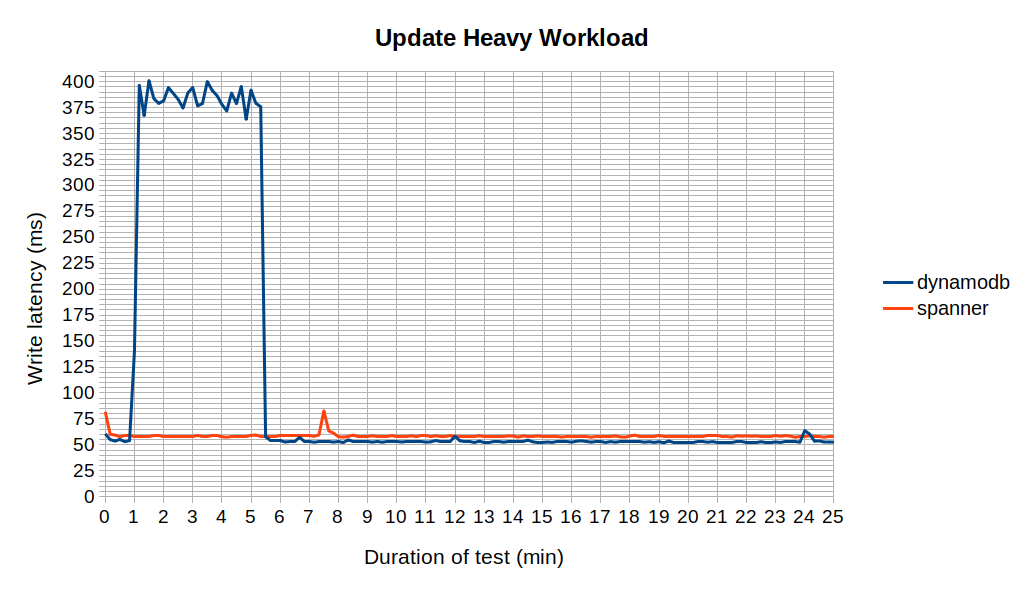
\includegraphics[width=0.47\textwidth]{workloadA_size300.png}}
\caption{Line Chart for Executing Update Heavy Workload (field size 300 bytes)}
\label{fig:workloadA_size300}
\end{figure}  
 
\begin{figure}[h]
\centering
\fbox{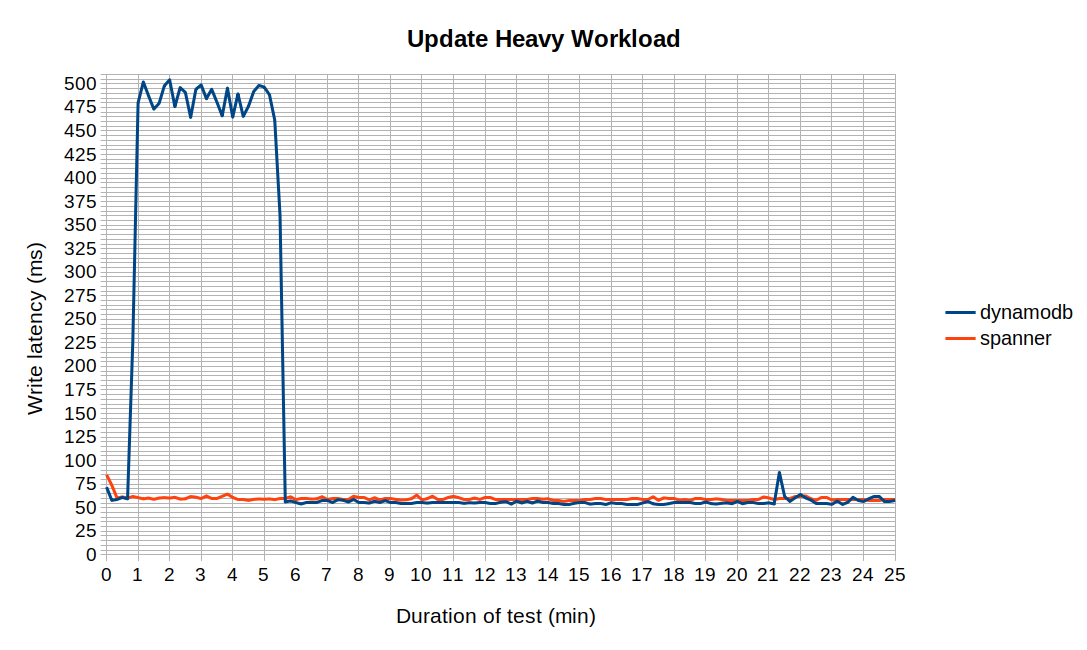
\includegraphics[width=0.47\textwidth]{workloadA_size500.png}}
\caption{Line Chart for Executing Update Heavy Workload (field size 500 bytes)}
\label{fig:workloadA_size500}
\end{figure}  

It is immediately noticeable that when the size of the record increases, the performance of DynamoDB starts to gradually decline. The same latency spikes that we observed in figure \ref{fig:workloadA_size100} are present here but this time they are even larger. For instance, there is a spike from 50-60 ms up to 400ms for the 3kB record size and one from 50-60ms up to 500ms for the 5kB records. Also, the box plots - figure \ref{fig:workloadA_size300} and \ref{fig:boxplot_size500} - clearly demonstrate that the performance of Google Spanner is way more stable and although the record size increases, Spanner's write latency remains approximately the same throughout all the experiments. In other words, although DynamoDB demonstrated lower latency (i.e lower with close to 10 milliseconds) in the first experiment, Google Spanner started "catching up" as soon as the record size increased. The whiskers in the box plots show that the range of latencies Spanner displays is significantly more narrow than the one of DynamoDB - i.e. the variance and the standard deviation for the Spanner measurements are considerably smaller. This speaks unequivocally that Spanner has more stable and reliable performance than DynamoDB. 

\begin{figure}[h]
\centering
\fbox{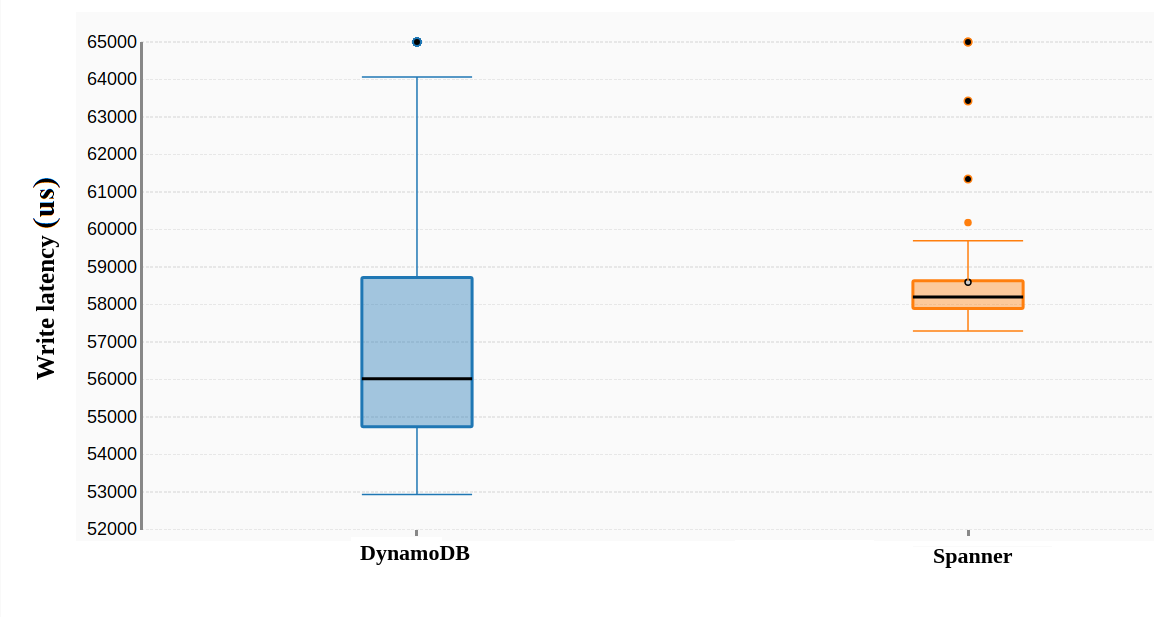
\includegraphics[width=0.47\textwidth]{boxplotA_size300.png}}
\caption{Box Plot for Executing Update Heavy Workload (field size 300 bytes)}
\label{fig:boxplot_size300}
\end{figure} 
 
\begin{figure}[h]
\centering
\fbox{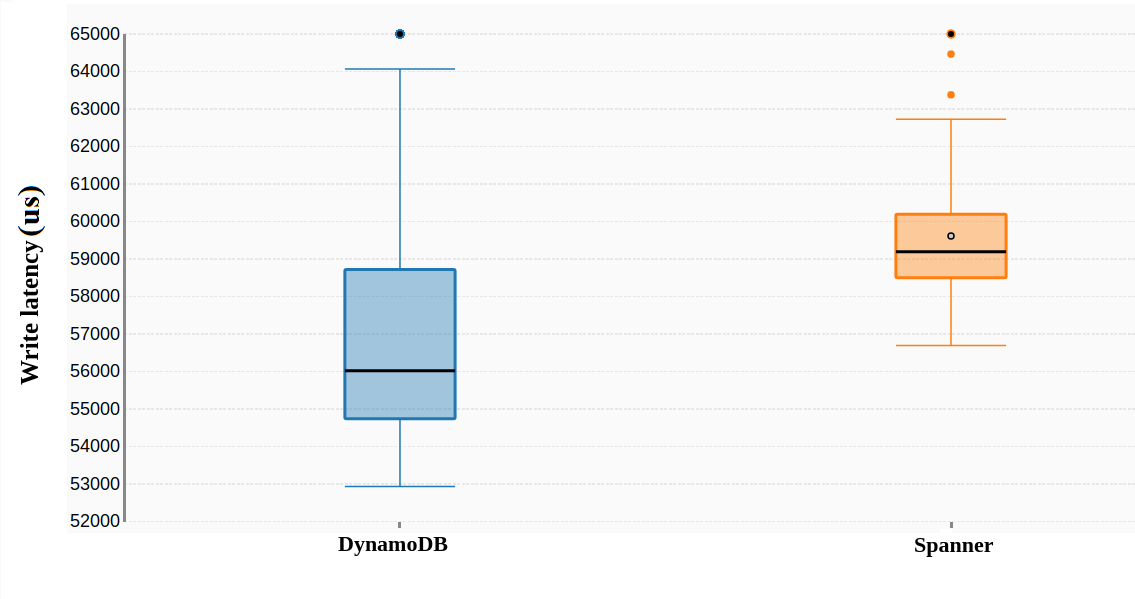
\includegraphics[width=0.47\textwidth]{boxPlotA_size500.png}}
\caption{Box Plot for Executing Update Heavy Workload (field size 500 bytes)}
\label{fig:boxplot_size500}
\end{figure} 

\subsection{Update Heavy Workload (field size 1000 bytes):}
 The last experiment that we ran was with records of 10kB size. The results in that case showed the most dramatic increase in latencies for DynamoDB. Figures \ref{fig:workloadA_size1000} and \ref{fig:boxplot_size1000} clearly support this claim.
 
\begin{figure}[h]
\centering
\fbox{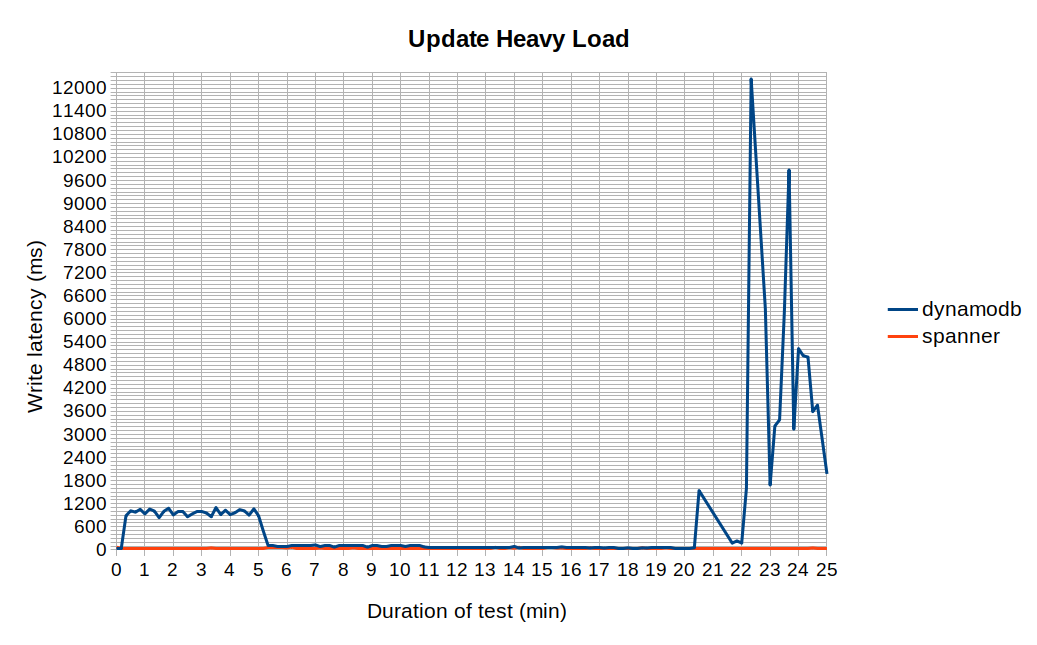
\includegraphics[width=0.47\textwidth]{workloadA_size1000.png}}
\caption{Line Chart for Executing Update Heavy Workload (field size 1000 bytes)}
\label{fig:workloadA_size1000}
\end{figure}  

\begin{figure}[h]
\centering
\fbox{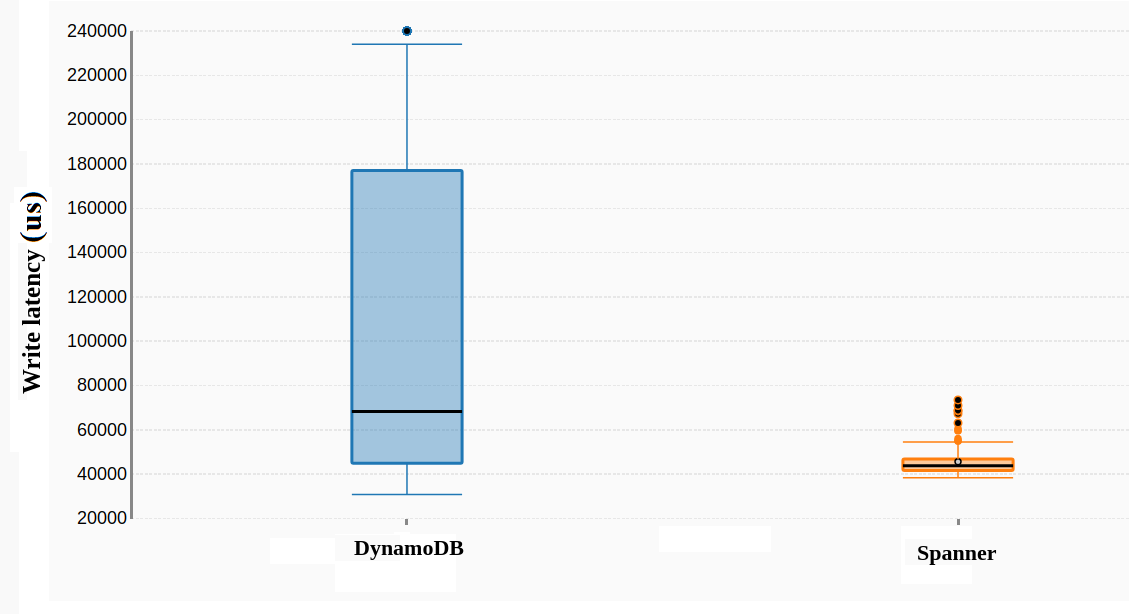
\includegraphics[width=0.47\textwidth]{boxPlotA_size1000.png}}
\caption{Box Plot for Executing Update Heavy Workload (field size 1000 bytes)}
\label{fig:boxplot_size1000}
\end{figure}    

The first noteworthy difference from the previous experiments was that this time DynamoDB had higher latencies than Spanner throughout the whole benchmark run. Also, not only did the trend for unstable performance continue to occur, but the write latency spikes became unacceptable from the client's perspective. To be more specific, at around the 22 minute mark, DynamoDB was executing an update operations with latency of 12 seconds. Additionally, box plot \ref{fig:boxplot_size1000}, shows that as stated in the section for the previous experiments, Spanner not only caught up with DynamoDB, but it also got significantly ahead. In fact, the whole Spanner "box" (with the exception of the outliers) fits under the median of DynamoDB's measurements. In statistical terms, this means that in 50\% of the cases throughout the experiment, DynamoDB was slower than Spanner. These results were quite surprising for us, given that we are comparing an eventually consistent (i.e. DynamoDB) with a strongly consistent store (i.e. Spanner). Unfortunately, given the fact both stores do not offer a closer look "behind the scenes" and we operate with them as if they are a black box, it is extremely challenging to make a conclusive statement about the reasons behind the observed performance. However, since the maximum record size for DynamoDB is 400kB - i.e. nowhere near the sizes that we ran tests with - it is quite possible that the DynamoDB shortcomings that we observed are caused not by any performance "deficiency" but rather  by the type of DynamoDB deployment that we used. In other words, it is very likely that if we use high reserved read/write capacities, DynamoDB might perform considerably better.

\section{CONCLUSION}
With the information presented in the previous sections and the measurements obtained in the scope of the project, we can finally go back to the research questions introduced in the beginning of this report and try to answer them. The questions were:
\begin{itemize}
    \item What is AWS DynamoDB and Google Spanner’s write performance in terms of latency when both stores are introduced with update heavy workloads? 
    \item How does the database record size affect the write latency of the two stores?  
\end{itemize}
Honestly, to answer the first question without touching the second one would result in an inaccurate statement. All in all, both stores performed well when dealing with update heavy workloads and demonstrated low write latencies for records of size 1kB. That being the case, when we address the second part of the question, with the increasing record size, the write latencies of one of the stores changed significantly. As discussed in the "Results" section, with the gradual increase in the record field size (and as consequence the overall record size) DynamoDB's latencies increased as well. This finding was really unexpected when considering the fact that DynamoDB is a eventually consistent store while Google Spanner aims at strong consistency. In addition, we used record sizes that are not near the documented maximum capabilities of the two stores, which makes the experiment outcome even more unforeseen.
As mentioned multiple times throughout the text, one possible explanation of the encountered results is the free-tier deployment of DynamoDB. Altough, at this point in time we did not have the financial means to run a highly provisioned instance, it is reasonable to assume that with certain amount of "reserved" read/write capacities DynamoDB will have a more stable performance. \par
With this in mind, the answer to the research questions can be summarized as follows:
Both stores have decently low write latencies (i.e. 50-60 ms) when dealing with update heavy workloads and the record size is small (i.e. close to 1kB). Nevertheless, when the record size increases, DynamoDB's performance drops whereas Google Spanner continues to maintain constantly small write latency. \par
With that said, it is not a trivial task to take a final stand and claim that Spanner's write performance in terms of latency will continue to stay stable and the performance of DynamoDB will continue to decline when the record size increases up to 400kB - the item size limit for Dynamo. To be completely honest, although the collected measurements presented some unambiguous trends,  comparing the two stores remains extremely challenging because of their "black-box" nature. That is why will keep a more conservative position by not announcing whether or not the presented results are unequivocal proof that Spanner performs better than DynamoDB under update heavy workloads. 


\addtolength{\textheight}{-12cm}   % This command serves to balance the column lengths

 
 

\printbibliography

\section{Additional Visual Material}
The following figures present the measurements we took for update heavy workloads with record field size of 100 bytes at different times of the day.
\begin{figure}[h]
\centering
\fbox{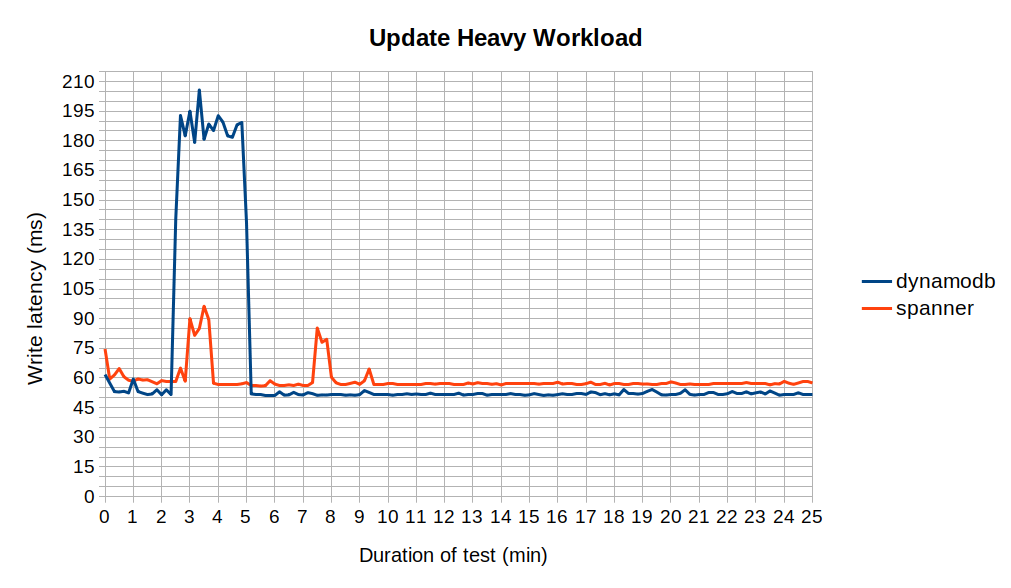
\includegraphics[width=0.47\textwidth]{workloadA_2nd-Run_chart.png}}
\caption{Line Chart for Executing Update Heavy Workload early in the morning (field size 100 bytes)}
\label{fig:workloadA_morning}
\end{figure}  

\begin{figure}[h]
\centering
\fbox{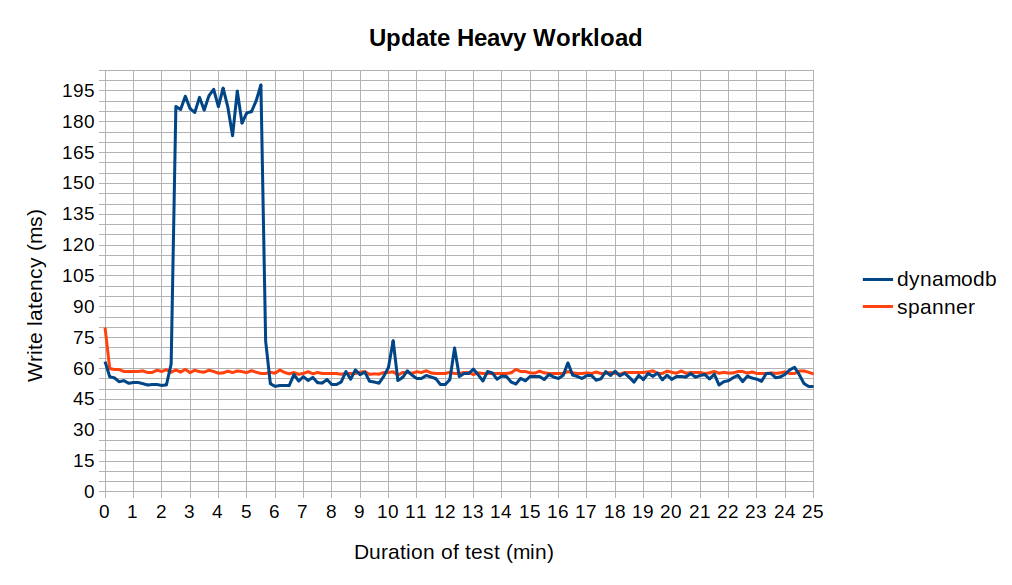
\includegraphics[width=0.47\textwidth]{workloadA_3rd-Run_chart.png}}
\caption{Line Chart for Executing Update Heavy Workload late in the night (field size 100 bytes)}
\label{fig:workloadA_night}
\end{figure}  

Lastly, figures \ref{fig:workloadEChart} and \ref{fig:workloadEBox} below show how the two data stores performed for loads that were not directly related to the research questions. More specifically, we tested how both stores will perform for hot-key workloads:
\begin{figure}[h]
\centering
\fbox{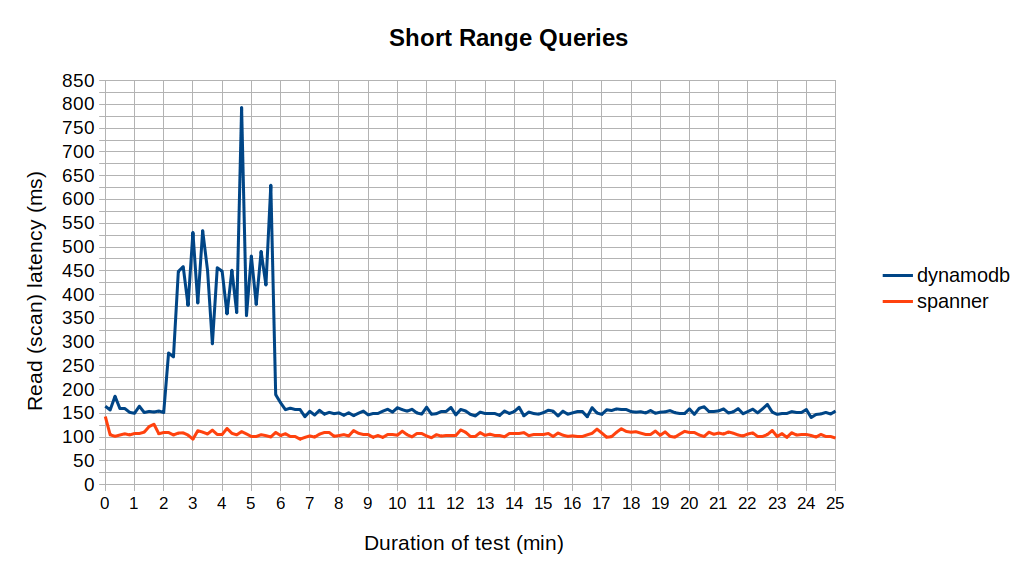
\includegraphics[width=0.47\textwidth]{workloadE_chart.png}}
\caption{Line Chart for Executing Short Range Queries}
\label{fig:workloadEChart}
\end{figure}  

\begin{figure}[h]
\centering
\fbox{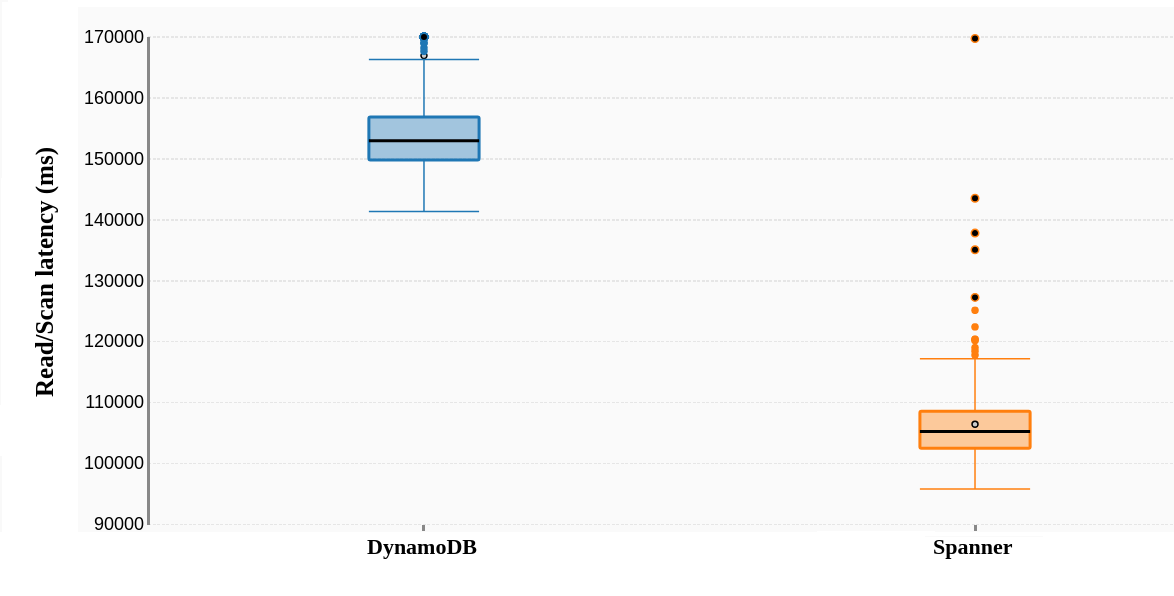
\includegraphics[width=0.47\textwidth]{boxPlotE.png}}
\caption{Box Plot for Executing Short Range Queries}
\label{fig:workloadEBox}
\end{figure}  
\end{document}
